% Chapter Template

% Main chapter title
%\chapter[toc version]{doc version}
\chapter{Background}

% Short version of the title for the header
%\chaptermark{version for header}

% Chapter Label
% For referencing this chapter elsewhere, use \ref{ChapterTemplate}
\label{chp:background}

% Write text in here
% Use \subsection and \subsubsection to organize text

\section{Introduction}
\label{sec:background_intro}
We will use deep neural networks and probabilistic models extensively throughout this thesis. Although the basic concepts of the former should be fairly familiar to most readers, the latter might be less widely known. Moreover, some of the tools and algorithms that we are going to use are not so trivial and therefore they should better be introduced first, for the sake of completeness and readability.

This chapter will then focus on providing a brief yet rigorous background on the aforementioned subject. We shall start by clarifying some notation and conventions we shall adopt (\Secref{sec:definitions}). Then we proceed with a short introduction to Bayesian networks, motivated by the factorization properties of joint probability functions (\Secref{}). Expectation-Maximization (EM) is presented as an efficient algorithm to learn probabilistic models with unobserved variables (\Secref{}). We then review the hidden Markov model (HMM), which will play a central role in Chapter \ref{chp:networked_data_streams}, and present the instantiation of the EM algorithm for this particular model (\Secref{}). The chapter is concluded with a brief introduction to variational inference (\Secref{}). Under this setting, the variational autoencoder will deserve special attention (\Secref{}), as it will be one of the models employed in Chapter \ref{chp:domain_generalization}.

\section{Useful definitions and conventions}
\label{sec:definitions}
In this section, we introduce some further notations and definitions that will be used throughout this document.

It is important to remark that the same notation is used to denote discrete and continuous random variables as well as to denote probability mass functions and probability density functions. Specifically, given a random variable $\rx$ defined in $\gX$, $p(\rx)$ denotes the probability mass of $\rx$, if $\gX$ is discrete, or the probability density of $\rx$, otherwise. In either case, the \emph{support} of $p(\rx)$ is defined as $\mathrm{Supp}(p(\rx)) \triangleq \lbrace x \in \gX: p(\rx=x) > 0 \rbrace$. Moreover, when we want to denote the probability (density) of some arbitrary but fixed value $x \in \gX$, we often use $p(x)$ as a short for $p(\rx=x)$.

The joint probability function of $\rx$ and $\ry$ is denoted by $p(\rx,\ry)$ and the corresponding conditionals of $\ry$ given $\rx$ and $\rx$ given $\ry$ are denoted by the usual $p(\ry \mid \rx)$ and $p(\rx \mid \ry)$, respectively. Again, $\rx$ and $\ry$ can be both discrete, both continuous, or one continuous and the other discrete. For three or more random variables the notation generalizes naturally.

The marginalization of $p(\rx,\ry)$ with respect to a discrete $\ry$ is written as:
\begin{equation}
    \sum_{\ry} p(\rx,\ry) \triangleq \sum_{y \in \gY} p(\rx,y) = p(\rx),
\end{equation}
and the marginalization of $p(\rx,\ry)$ with respect to a continuous $\rx$ is written as:
\begin{equation}
    \int p(\rx,\ry) \d \rx \triangleq \int_{\gX} p(x,\ry) \d x = p(\ry).
\end{equation}
Note that for brevity we omit the domain of the summation or integration, as this is defined implicitly by the set where the random variable is defined. The integral notation is also used for the marginalization with respect to random variables whose type is unspecified. Similarly, if $f(\rx)$ is a function of a random variable $\rx$,
\begin{equation}
    \sum_\rx f(\rx) \triangleq \sum_{x \in \gX} f(x) \quad \text{or} \quad \int f(\rx) \d \rx \triangleq \int_\gX f(x) \d x,
\end{equation}
depending on whether $\rx$ is discrete or continuous, respectively. Hence, we can write the \emph{expectation} of $f(\rx)$ with respect to $p(\rx)$ as:
\begin{equation}
    \E_{\rx \sim p(\rx)} \left[f(\rx)\right] \triangleq \sum_\rx f(\rx) p(\rx) \quad \text{or} \quad \E_{\rx \sim p(\rx)} \left[f(\rx)\right] \triangleq \int f(\rx) p(\rx) \d \rx,
\end{equation}
for a discrete or continuous $\rx$, respectively.

\section{Bayesian networks}
\label{sec:bayesian_networks}

\subsection{Definition and structural properties}
\label{sec:bayesian_net_definition}

Given $n$ random variables $\rx_1, \rx_2, \dots, \rx_n$, the \emph{chain rule of probability} allows the factorization of their joint distribution as:\footnote{The expression on the right-hand side of \eqref{eq:chain_rule} is not well defined outside the support of $p(\rx_1), p(\rx_1, \rx_2), \dots, p(\rx_1, \rx_2, \dots, \rx_{n-1})$. For those values, one has $p(\rx_1, \rx_2, \dots, \rx_n)=0$.}
\begin{equation}
    \label{eq:chain_rule}
    p(\rx_1,\rx_2,\dots,\rx_n) = p(\rx_1) \prod_{i=1}^n p(\rx_i \mid \rx_{1}, \rx_{2}, \dots, \rx_{i-1}).
\end{equation}
Starting from this product, we may build a directed graph $\gG$ with $n$ vertices, one for each random variable, where there exists an edge $i \rightarrow j$ if and only if there is a factor where $\rx_i$ is conditioned on $\rx_j$. Such a graph is known as a \emph{Bayesian network}. From its definition, it is clear that the factorization in \eqref{eq:chain_rule} corresponds to the graph in \Figref{fig:complete_bayesian_net}. Clearly, a Bayesian network defines a bijection between random variables and graph nodes, so with a slight abuse of terminology we represent and refer to nodes by the random variable they are associated with, rather than by their index.

\begin{figure}
    \centering
    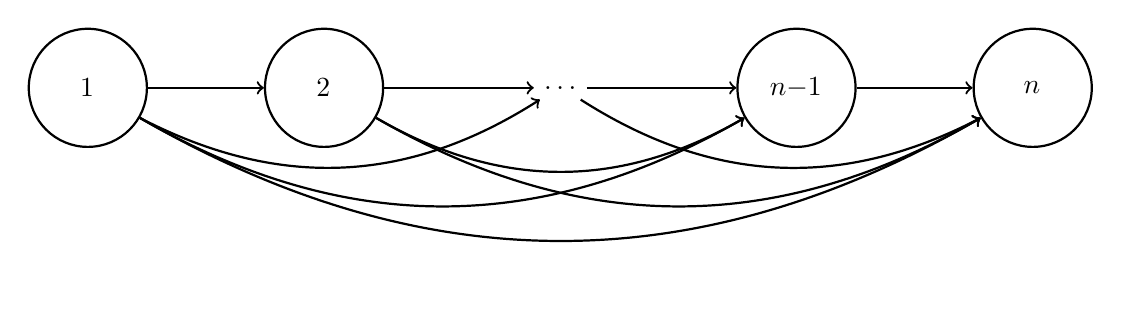
\begin{tikzpicture}[auto, node distance=3cm, every loop/.style={},thick,
        main node/.style={circle,draw,font=\sffamily\Large\bfseries},
        hidden node/.style={circle,draw,fill=lightgray,font=\sffamily\Large\bfseries},
        box node/.style={rectangle,dashed,draw,anchor=center},
        empty node/.style={rectangle,fill=white,anchor=center},]


        \node[main node,minimum size=1.5cm] (x1) {$\rx_1$};
        \node[main node,minimum size=1.5cm] (x2) [right of=x1] {$\rx_2$};
        \node[empty node] (dots) [right of=x2] {$\dots$};
        \node[main node,minimum size=1.5cm] (xn_1) [right of=dots] {$\rx_{n-1}$};
        \node[main node,minimum size=1.5cm] (xn) [right of=xn_1] {$\rx_n$};


        \draw[->]
        (x1) edge (x2)
        (x2) edge (dots)
        (dots) edge (xn_1)
        (xn_1) edge (xn)
        (x1) edge[bend right] (dots)
        (x1) edge[bend right] (xn)
        (x1) edge[bend right] (xn_1)
        (x2) edge[bend right] (xn_1)
        (x2) edge[bend right] (xn)
        (dots) edge[bend right] (xn);

    \end{tikzpicture}
    \caption{A complete Bayesian network.}
    \label{fig:complete_bayesian_net}
\end{figure}

Since the factorization in \eqref{eq:chain_rule} is general (i.e.\ it does not assume any conditional independence between random variables), the Bayesian network in \Figref{fig:complete_bayesian_net} is said to be \emph{complete}. When conditional independences are present, the graph becomes sparser. For instance, for all $i \geq 3$, $\rx_i$ is conditionally independent of $\rx_{1}, \rx_{2}, \dots, \rx_{i-2}$ given $\rx_{i-1}$, then $p(\rx_i \mid \rx_{1}, \rx_{2}, \dots, \rx_{i-1}) = p(\rx_i \mid \rx_{i-1})$ and thus the Bayesian network reduces to the \emph{chain} represented in \Figref{fig:chain_bayesian_net}.

\begin{figure}
    \centering
    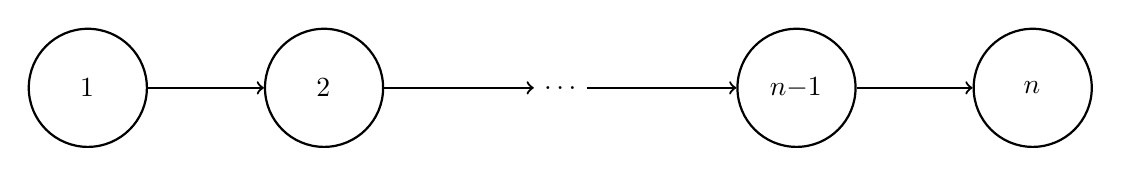
\begin{tikzpicture}[auto, node distance=3cm, every loop/.style={},thick,
        main node/.style={circle,draw,font=\sffamily\Large\bfseries},
        hidden node/.style={circle,draw,fill=lightgray,font=\sffamily\Large\bfseries},
        box node/.style={rectangle,dashed,draw,anchor=center},
        empty node/.style={rectangle,fill=white,anchor=center},]


        \node[main node,minimum size=1.5cm] (x1) {$\rx_1$};
        \node[main node,minimum size=1.5cm] (x2) [right of=x1] {$\rx_2$};
        \node[empty node] (dots) [right of=x2] {$\dots$};
        \node[main node,minimum size=1.5cm] (xn_1) [right of=dots] {$\rx_{n-1}$};
        \node[main node,minimum size=1.5cm] (xn) [right of=xn_1] {$\rx_n$};


        \draw[->]
        (x1) edge (x2)
        (x2) edge (dots)
        (dots) edge (xn_1)
        (xn_1) edge (xn);;
    \end{tikzpicture}
    \caption{A chain.}
    \label{fig:chain_bayesian_net}
\end{figure}
An important property of Bayesian networks is the fact that they are always directed \emph{acyclic} graphs. The non-existence of loops allows us to recover the factorization of the joint distribution by examining the structure of the graph $\gG$ and applying the formula:
\begin{equation}
    p(\rx_1, \rx_2, \dots, \rx_n) = \prod_{i=1}^n p(\rx_i \mid \parents_\gG(\rx_i)),
\end{equation}
where $\parents_\gG(\rx_i)$ are the parents of the node $\rx_i$ in the graph $\gG$. It is important to highlight that, although there is a one-to-one correspondence between a factorization of a joint distribution into conditional distributions and a Bayesian network, the same joint distribution can sometimes be factorized in multiple different but equivalent forms, each one corresponding to a different Bayesian network. This is the case of \emph{chains} and \emph{forks}, which we discuss next.

\subsection{Chains and forks}
\label{sec:chains_forks}
Let us consider the case where we have three random variables $\rx_1, \rx_2, \rx_3$ and assume that $\rx_1$ and $\rx_3$ are independent given $\rx_2$. Under this setting, we have:
\begin{align}
    p(\rx_1, \rx_2, \rx_3) &= p(\rx_1) p(\rx_2 \mid \rx_1) p(\rx_3 \mid \rx_2) \label{eq:chain}\\
    &= p(\rx_2) p(\rx_1 \mid \rx_2) p(\rx_3 \mid \rx_2) \label{eq:fork}\\
    &= p(\rx_3) p(\rx_2 \mid \rx_3) p(\rx_1 \mid \rx_2) \label{eq:reversed_chain}
\end{align}
The three equivalent factorizations \plaineqref{eq:chain} -- \plaineqref{eq:reversed_chain} correspond, from left to right, to the three Bayesian networks in \Figref{fig:equiv_bayesian_nets}.

\begin{figure}
    \centering
    \begin{subfigure}[t]{0.32\textwidth}
        \resizebox{\textwidth}{!}{
        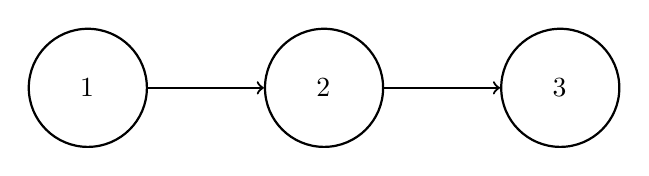
\begin{tikzpicture}[auto, node distance=3cm, every loop/.style={},thick,
            main node/.style={circle,draw,font=\sffamily\Large\bfseries},
            hidden node/.style={circle,draw,fill=lightgray,font=\sffamily\Large\bfseries},
            box node/.style={rectangle,dashed,draw,anchor=center},
            empty node/.style={rectangle,fill=white,anchor=center},]


            \node[main node,minimum size=1.5cm] (x1) {$\rx_1$};
            \node[main node,minimum size=1.5cm] (x2) [right of=x1] {$\rx_2$};
            \node[main node,minimum size=1.5cm] (x3) [right of=x2] {$\rx_{3}$};

            \draw[->]
            (x1) edge (x2)
            (x2) edge (x3);
        \end{tikzpicture}}
        \caption{A three-variable chain.}
        \label{fig:3var_chain_bayesian_net}
    \end{subfigure}
    \begin{subfigure}[t]{0.32\textwidth}
        \resizebox{\textwidth}{!}{
        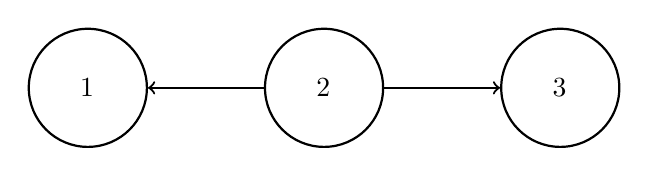
\begin{tikzpicture}[auto, node distance=3cm, every loop/.style={},thick,
            main node/.style={circle,draw,font=\sffamily\Large\bfseries},
            hidden node/.style={circle,draw,fill=lightgray,font=\sffamily\Large\bfseries},
            box node/.style={rectangle,dashed,draw,anchor=center},
            empty node/.style={rectangle,fill=white,anchor=center},]
            \node[main node,minimum size=1.5cm] (x1) {$\rx_1$};
            \node[main node,minimum size=1.5cm] (x2) [right of=x1] {$\rx_2$};
            \node[main node,minimum size=1.5cm] (x3) [right of=x2] {$\rx_{3}$};
            \draw[->]
            (x2) edge (x1)
            (x2) edge (x3);
        \end{tikzpicture}}
        \caption{A fork.}
        \label{fig:fork_bayesian_net}
    \end{subfigure}
    \begin{subfigure}[t]{0.32\textwidth}
        \resizebox{\textwidth}{!}{
        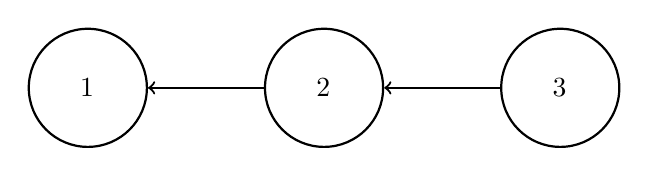
\begin{tikzpicture}[auto, node distance=3cm, every loop/.style={},thick,
            main node/.style={circle,draw,font=\sffamily\Large\bfseries},
            hidden node/.style={circle,draw,fill=lightgray,font=\sffamily\Large\bfseries},
            box node/.style={rectangle,dashed,draw,anchor=center},
            empty node/.style={rectangle,fill=white,anchor=center},]


            \node[main node,minimum size=1.5cm] (x1) {$\rx_1$};
            \node[main node,minimum size=1.5cm] (x2) [right of=x1] {$\rx_2$};
            \node[main node,minimum size=1.5cm] (x3) [right of=x2] {$\rx_{3}$};

            \draw[->]
            (x3) edge (x2)
            (x2) edge (x1);
        \end{tikzpicture}}
        \caption{A three-variable reversed chain.}
        \label{fig:revchain_bayesian_net}
    \end{subfigure}
    \caption{Equivalent three-variable Bayesian networks.}
    \label{fig:equiv_bayesian_nets}
\end{figure}

\subsection{Immoralities}
\label{sec:immoralities}